%\begin{document}
\chapter{湖试数据处理及分析}
本文研究水声相干通信的信号处理,重点研究了克服码间干扰的Turbo均衡技术和软迭代信道估计两项关键的核心技术。为了充分地检验前面所做的工作,验证水声相干通信Turbo均衡的性能,于2012年12月份在千岛湖组织了湖泊试验,获得了大量的湖试原始数据,并且对试验的数据进行了处理和分析。


%==========================================================================
\section{湖试的准备和过程}
\subsection{发射数据的准备}
待发射的信源数据位随机生成的高斯白噪声二进制数据,经Turbo编码后再进行符号映射成QPSK调制符号,最后进行交织之后送到发射机。系统的参数如表\ref{tab:6.1}
\begin{table}[hbt]
  \centering
  \caption{T-TCM基本参数}
  \label{tab:6.1}
  \begin{threeparttable}
  \begin{tabular}{cc}
    \hline
    参数名称&参数值\\
    \hline
    分量编码器&$[23,35]$\\
    编码方式&Turbo码\\
    映射方式&QPSK\\
    交织器算法&伪随机交织器\\
    交织长度&1936\\
   \hline
  \end{tabular}
\end{threeparttable}
\end{table}
一组数据包含14帧,每一帧数据的内容都是一样的。为了获取充足的数据,在每一个测试地点,总共进行了10组数据的传输。
图\ref{fig:6.1}为映射之后的QPSK符号的星座图,将生成的QPSK符号结合发送符号序列,并通过采样和升余弦滚降之后,通过发射机发送出去。
\begin{figure}[htb]
  \begin{center}
    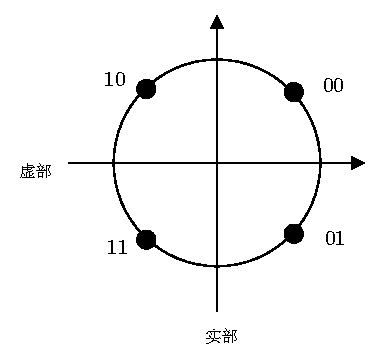
\includegraphics[width=0.8\textwidth]{images/qpsk.pdf}
  \end{center}
  \caption{QPSK符号映射星座图}
  \label{fig:6.1}
\end{figure}
\subsection{系统结构}
用于湖试的水声相干通信系统硬件框图如图\ref{fig:6.2}所示,
\begin{figure}[htb]
  \begin{center}
    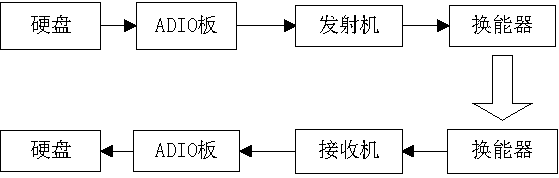
\includegraphics[width=0.9\textwidth]{images/block.pdf}
  \end{center}
  \caption{水声相干通信系统的结构框图}
  \label{fig:6.2}
\end{figure}
从图中可以看出,系统利用实验室研发的水声相干通信机进行数据的发射和接收,数据的生成和处理由PC机完成。
\subsection{试验布置}
试验的布置图见图\ref{fig:6.3}。试验使用新安江实验场的“实验1号”船作为接收母船(图\ref{fig:6.3}左上角),整个接收母船固定在距岸边$150$米左右的位置,水深$51$米。吊放换能器阵从接收母船的甲板吊放到水中,换能器阵上端距水面$10$米,下端距水面$21$米。
拖轮拖带“实验2号”船作为移动发射船(图\ref{fig:6.3}右上角),发射换能器拖曳在$5\textasciitilde10$米深度。在试验过程中移动发射船在距离接收母船$1000$米到$2600$米的范围内沿不同路线、以不同航速运动,发射不同类型的信号,来测试水声通信机的性能。
\begin{figure}[htb]
  \begin{center}
    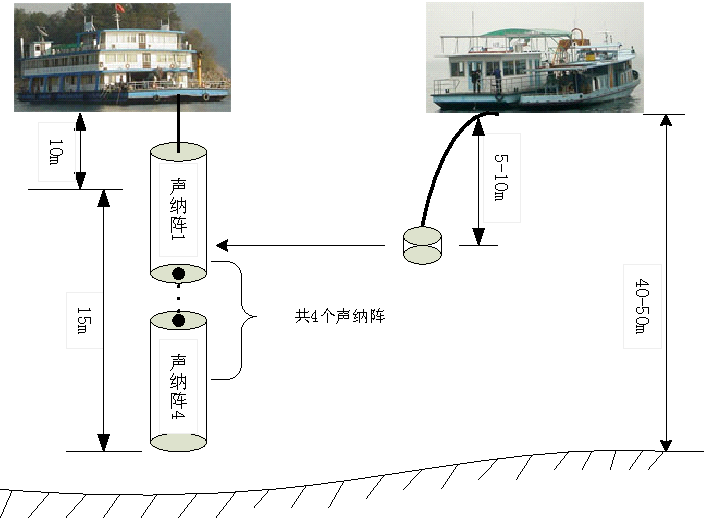
\includegraphics[width=0.9\textwidth]{images/trans.pdf}
  \end{center}
  \caption{湖试场地布置图}
  \label{fig:6.3}
\end{figure}
\subsection{湖试内容及环境}
湖试于2012年12月在千岛湖的中科院声学所新安江试验场进行,如图\ref{fig:6.1}。图中白色标记处为接收试验船抛锚位置,水深约50米,四个节点是移动发射船的三条航线,其中西南航线的最大距离为2617米,其他三条航线的距离从小到大依次为1052米、1645米和1736米。由于航线的目的是寻找通信网节点的合适位置,因此深度都在40~50米左右。
\begin{figure}[htb]
  \begin{center}
    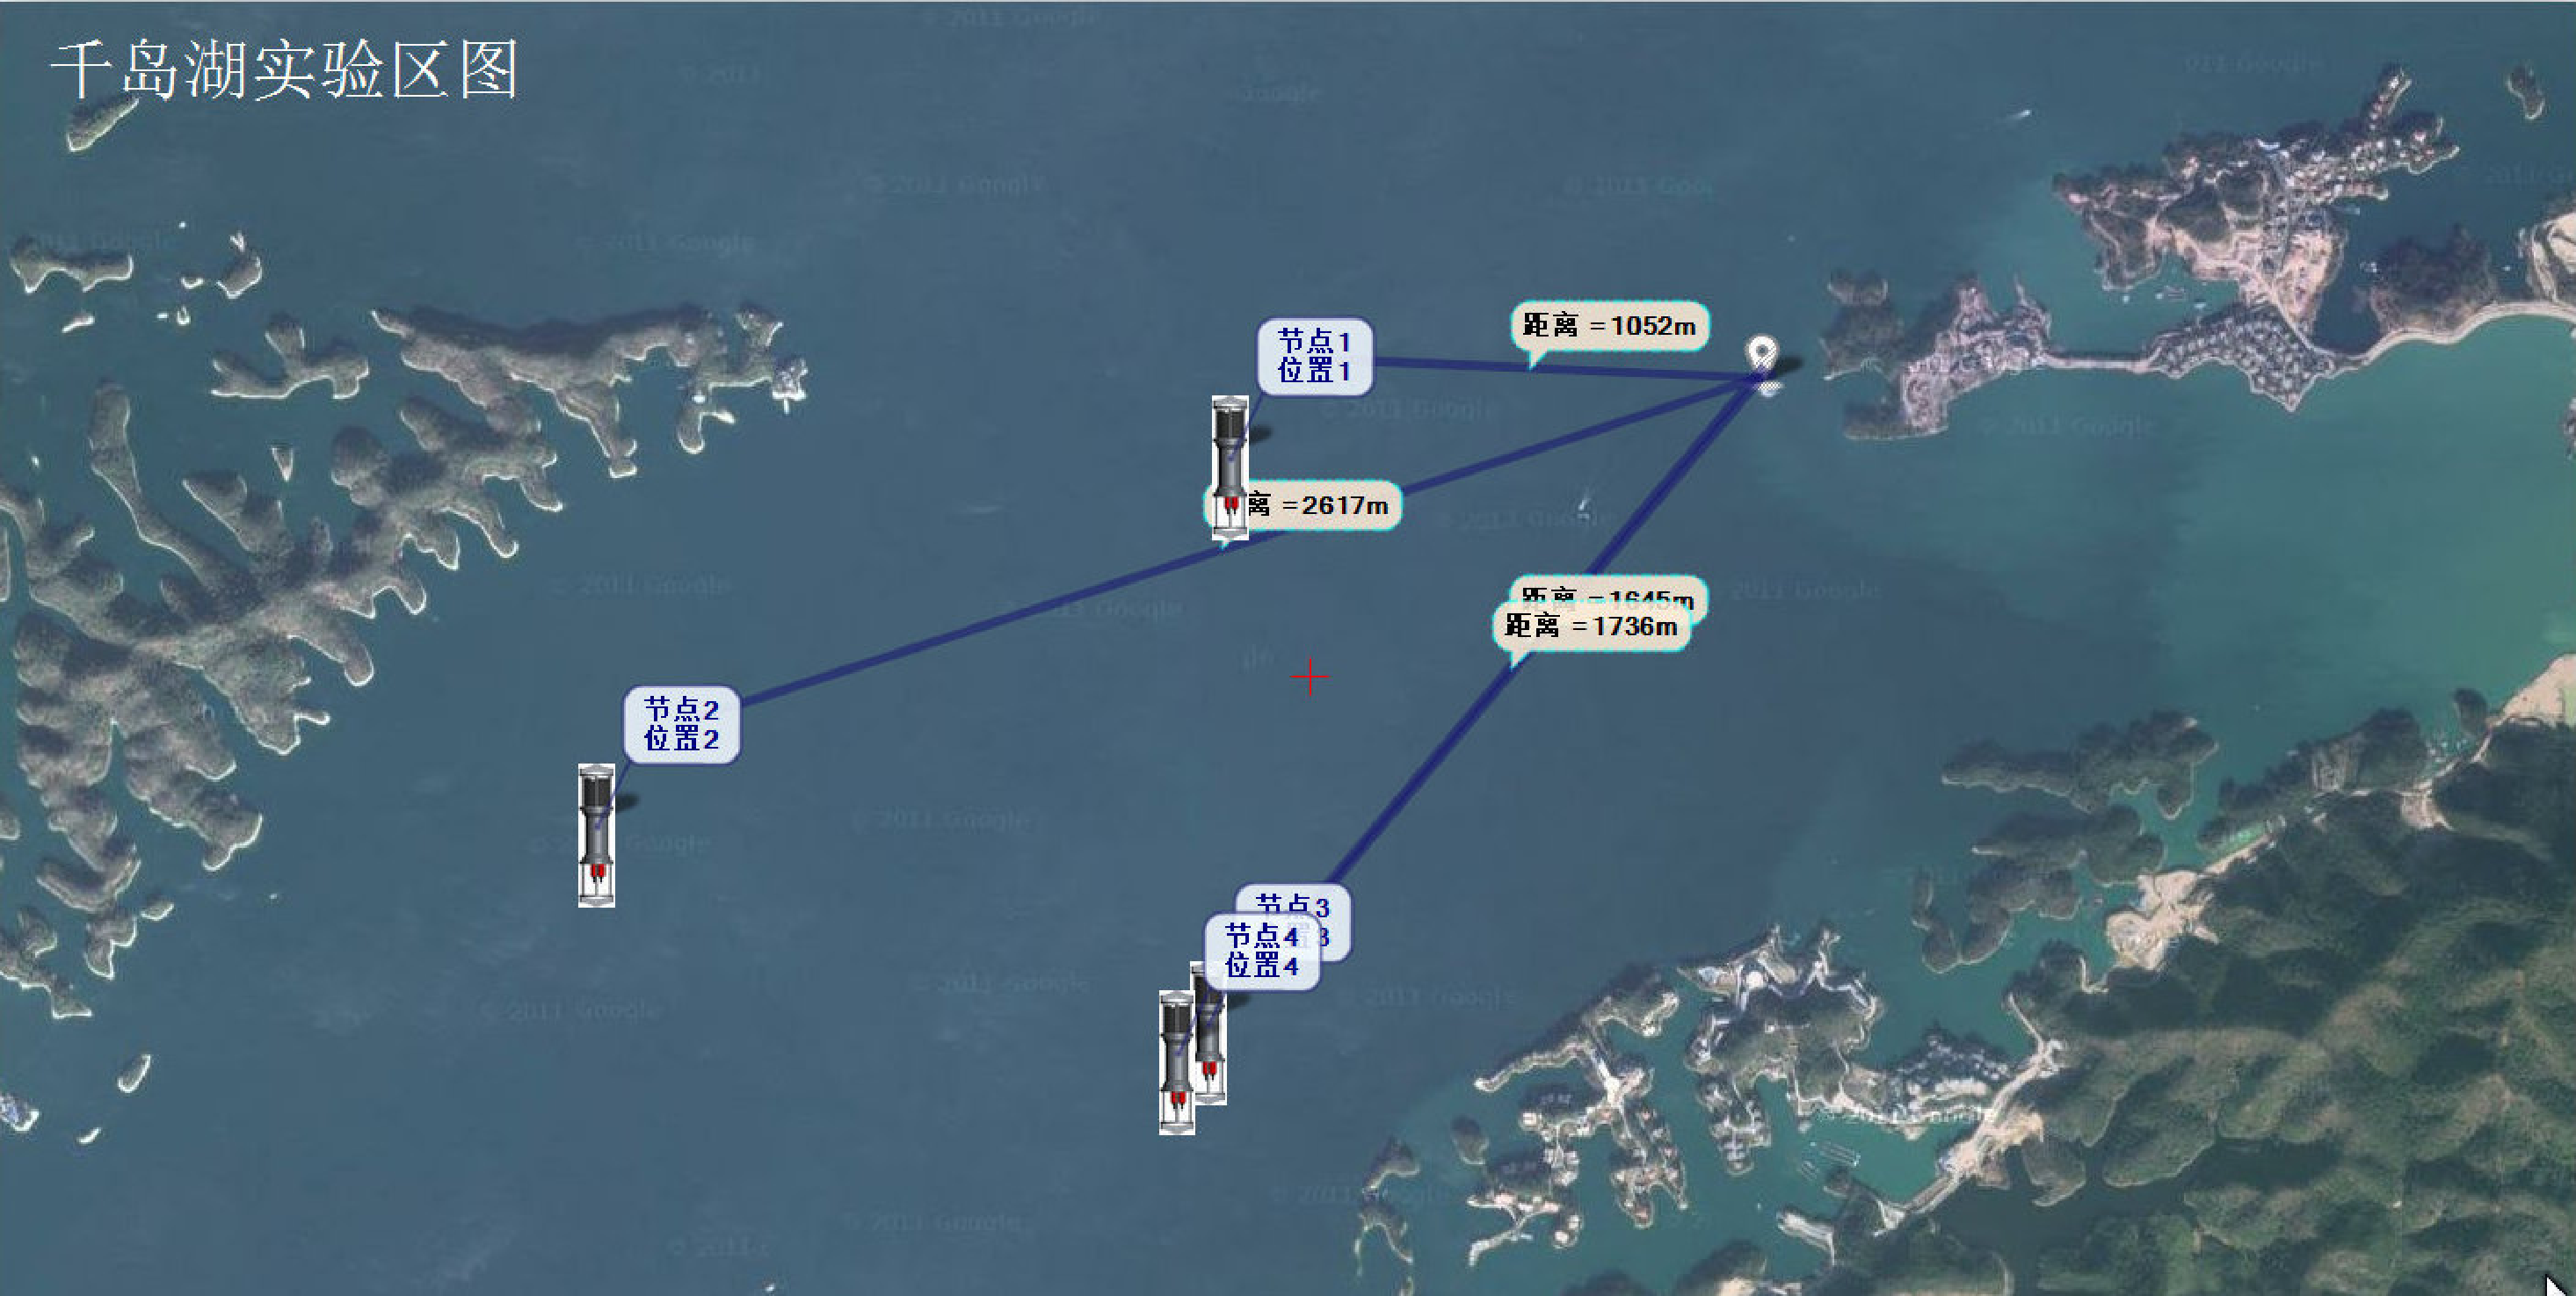
\includegraphics[width=0.9\textwidth]{images/exp.pdf}
  \end{center}
  \caption{千岛湖试验场示意图}
  \label{fig:6.4}
\end{figure}
从图\ref{fig:6.4}可以看出,航线的距离并不是有规律的设定的,原因有两点:1)此次试验主要是为了水声通信网的联网试验而准备的,因此,航线的距离并不是考虑的主要问题。2)当时风浪很大,船只到达指定节点投放位置之后并没有抛锚停下,而是随波逐流,此时,为了测试节点与母船通信畅通,耽搁了很长时间,这段时间可能导致了船只偏离指定位置。不过从图中可以看出,只有第三次和第四次发送数据时位置比较接近,其他的位置还是能够说明问题的。

与相对复杂的浅海相对比,湖试的信道情况更为复杂。由于通信水域是狭长的水道,两侧的山体和水下大量被淹没的小山的反射会产生比浅海更加复杂的多径结构。如果水声通信系统在这样信道条件下能够良好工作,那么其在浅海信道也能良好工作,在相对简单的深海信道中会有更好的性能。
\section{数据处理与分析}
\subsection{信道特性分析}
在此,利用声速剖面仪和温盐深测量仪在湖试现场采集的数据,并结合试验数据对声信道特性进行分析。
\subsubsection*{水温和声速}
图\ref{fig:6.5}是在湖试中测得的12月份千岛湖的温度剖面图和声速剖面图。千岛湖水体总体上来看,温差在5摄氏度左右,温度的变化对声速的影响还是非常明显的,但是仔细观察图\ref{fig:6.5}(a)中的温度剖面图可以发现,在深度$0\textasciitilde
30$米范围之内,温度的变化非常小,可以近似看做恒温的,而$30\textasciitilde
40$米深度范围时,温度变化比较大,而40米水深之后,温度又开始缓慢变化,基本可以看做是恒温的。
\begin{figure}[htb]
  \begin{center}
    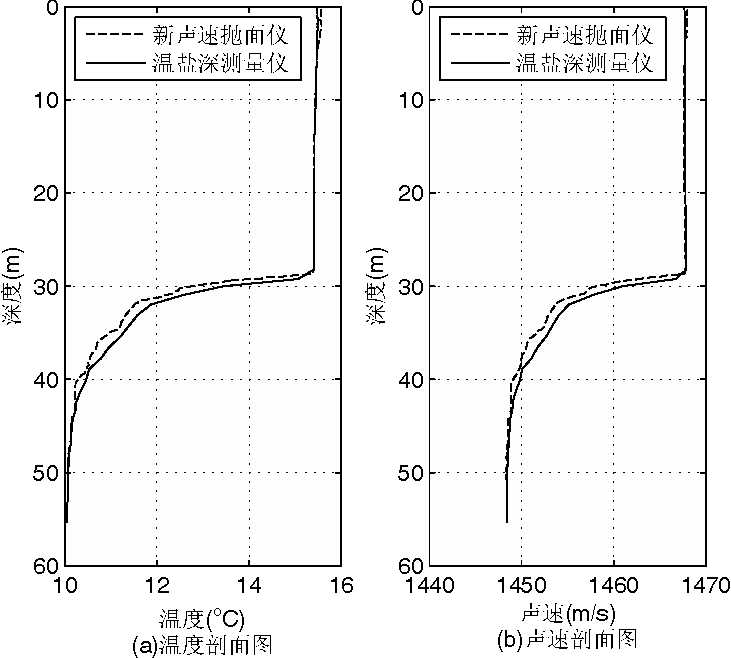
\includegraphics[width=0.9\textwidth]{images/speedTemp.pdf}
  \end{center}
  \caption{12月份千岛湖温度与声速剖面}
  \label{fig:6.5}
\end{figure}

现在观察图\ref{fig:6.5}(b)中的声速剖面,从图中可以看出,声速剖面和温度剖面是一一对应的,而本次试验时,接收机节点和发射机节点的位置都在$10\textasciitilde
30$之间。
\subsubsection*{信道冲激响应分析}
在水声通信机发射的信号中含有线性调频脉冲信号,见图\ref{fig:6.6}。线性调频脉冲信号的自相关函数具有窄的主瓣和低的旁瓣,可以近似看作一个冲激信号,则接收到额线性调频信号与线性调频信号的本地拷贝的互相关函数可以近似看成信道的冲激响应。
\begin{figure}[htb]
  \begin{center}
    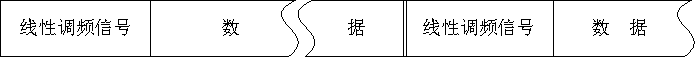
\includegraphics[width=0.9\textwidth]{images/frame.pdf}
  \end{center}
  \caption{发射信号数据帧组成结构}
  \label{fig:6.6}
\end{figure}
信道的冲激响应特性决定了水声通信系统接收机的结构以及自适应均衡算法的选择。湖试试验的最远距离为2617米,总共进行了四次数据发送的过程,图\ref{fig:6.7}给出了各个数据发送过程中12个通道的信道冲激响应。
\begin{figure}[htb]
  \begin{center}
    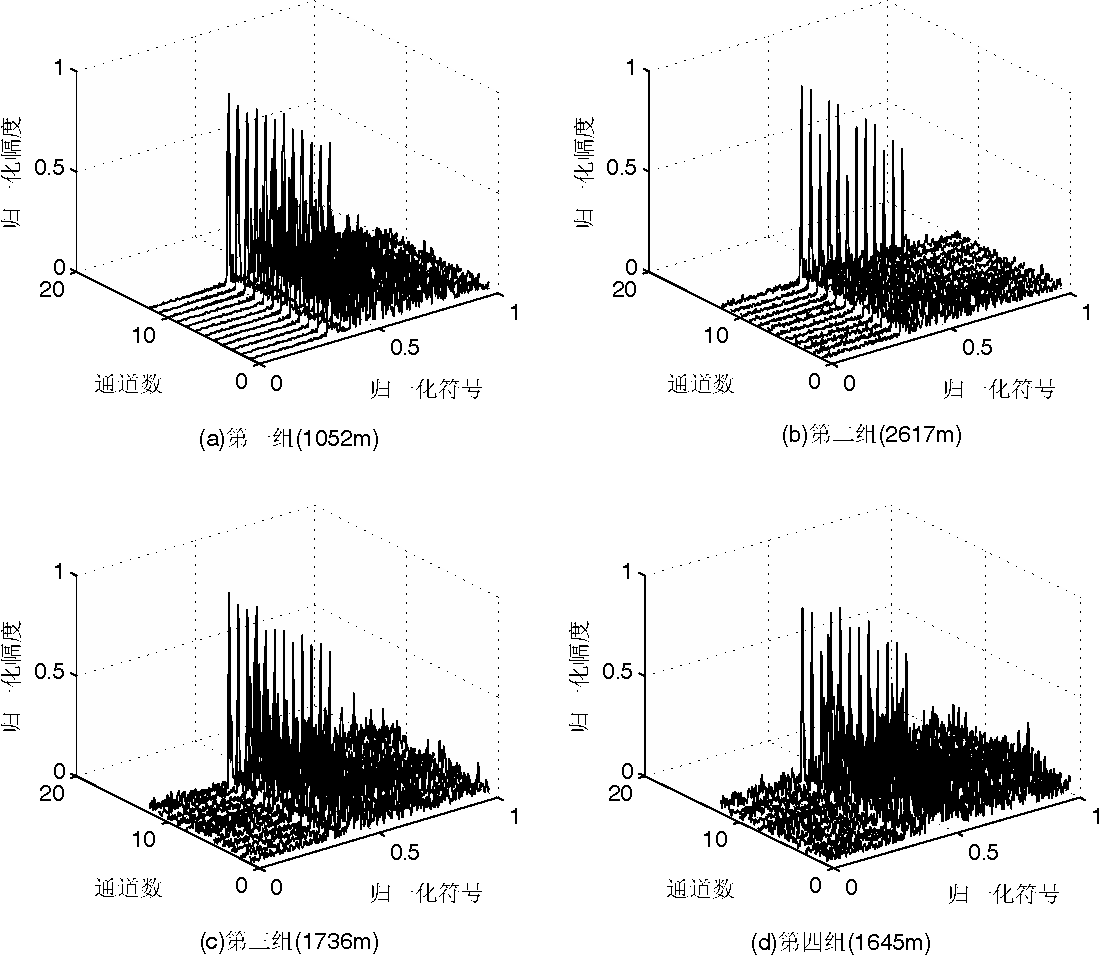
\includegraphics[width=\textwidth]{images/channelpulse.pdf}
  \end{center}
  \caption{不同距离水声信道冲激响应}
  \label{fig:6.7}
\end{figure}

下面来分析图\ref{fig:6.7}所示的信道冲激响应。在近距离时,各多径信号的时延较大,在所分析的时间窗口内仅有个别的强多径信号。随着距离的增大,多径信号的时延减小,越来越多的多次反射波进入时间窗,但其强度也越来越小。在所有的多径信号中,影响最大的是水面的一次反射波,其强度最大,与直达波在时间上最接近,容易造成同步脉冲检测不准。从图中看出第二组的时候,信道的特性最好,多径效应影响最小。

可以看出信道冲激响应随通信距离的不同而产生非常大的差异,相同距离不同时间的信道冲激响应也有明显差异,也就是说信道具有明显的时变特性。图\ref{fig:6.8}给出了1052米左右的距离上不同时间信道的冲激响应。图中X轴为不同数据帧(不同数据帧的发射时间是连连续的,因此可以表示时间的不同),Y轴是归一化符号,Z轴是相关函数的归一化模值。从图中可以看出,水声信道明显的多径结构和时变特性。
\begin{figure}[htb]
  \begin{center}
    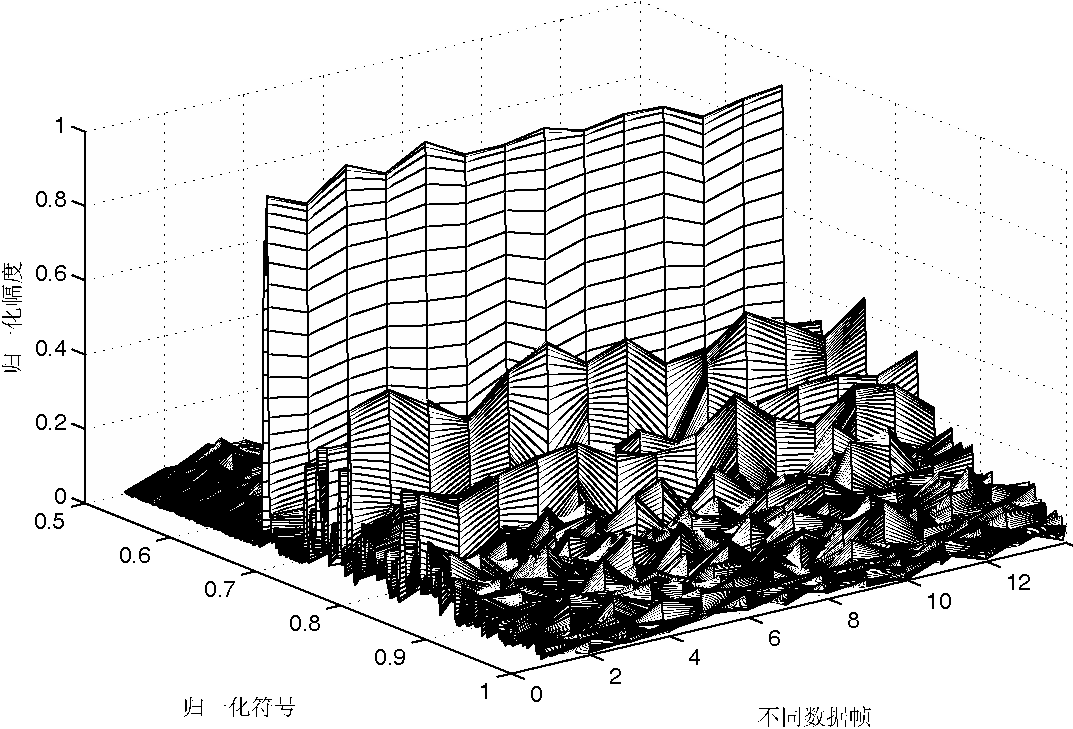
\includegraphics[width=0.9\textwidth]{images/channelTime.pdf}
  \end{center}
  \caption{1052m左右的距离上不同时间信道冲激响应}
  \label{fig:6.8}
\end{figure}
\subsection{接收数据的处理}
结合前面对湖试地点信道特性的分析,本节将给出Matlab实现的软迭代信道估计联合基于先验信息MMSE准则的线性Turbo均衡算法的湖试数据处理结果。

本文提出的线性Turbo均衡算法是单通道算法,而且为了处理数据的方便,湖试过程中,发送的每一组数据包中的每一帧数据都是一样的,因此处理的方式都是类似的。为了避免重复,只选取每个位置处两组数据包进行分析并给出其中一帧的处理结果。

\textbf{\sihao 2012年12月15日09:15:41数据 第一组} 

如图\ref{fig:6.9}为位置一(1052m)第一组第一帧的信道冲激响应以及误码率曲线,观察图\ref{fig:6.9}(a),信道冲激响应的多径比较严重,此处符号长度是归一化的结果,而归一化的长度为3073个符号,因此可以看出,多径的长度很长。此时,虽然本文提出的均衡算法在此种信道条件下实现无差错的译码,但是要求均衡器长度以及信道冲激响应的估计长度都很长,当均衡器长度为90,信道冲激响应的估计长度为86时,在均衡器迭代3次,译码器迭代1次时,可以实现无差错译码。但此时计算量非常大,在实际应用中很难满足要求。

在结合T-TCM码的Turbo均衡中,有两个迭代:一处为均衡器与译码器之间的迭代,此处成为外迭代,一处为译码器两个分量译码器之间的迭代,此处成为内迭代。从图\ref{fig:6.9}(b)可以得出两种迭代对误码率曲线的影响。横坐标表示的是均衡器的迭代次数,随着次数的增加,误码率曲线呈下降趋势。分析其原因在于,随着均衡器与译码器之间迭代次数的增加,外部信息越来越可靠,因此均衡和译码的性能越来越高。图中三条曲线代表着Turbo码的不同迭代次数的误码率性能,从图中可以看出,Turbo码内部的迭代次数的增加也能够提高均衡和译码性能,原因在于,Turbo内部迭代次数的增加能够使得译码器输出更可靠的外部信息,从而提高均衡性能。从图中还可以看出,相应的增加内迭代的次数可以降低外迭代次数而实现无差错译码,因此,为了获得最小的运算复杂度,需要平衡考虑两种迭代次数。

为了减少均衡器和相位估计器的长度,从而降低计算量,可以考虑将时间反转技术引入到Turbo均衡中,将多通道的数据时间反转并合并之后再通过本文提出的均衡算法,此时均衡和相位估计的长度大大降低,从而降低计算量。

\begin{figure}[htb]
  \begin{center}
    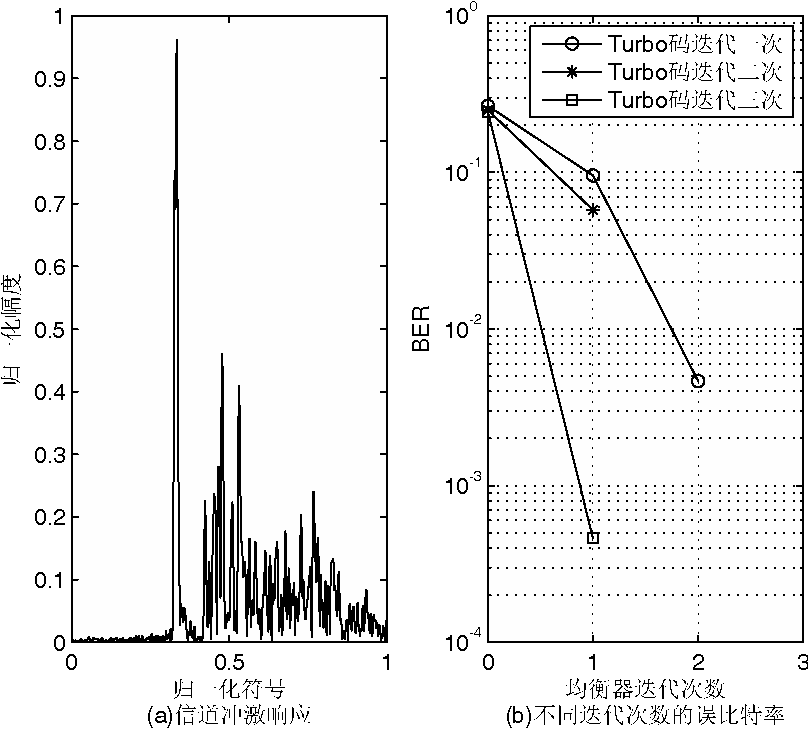
\includegraphics[width=0.9\textwidth]{images/result_1_1.pdf}
  \end{center}
  \caption{1052米处第一组数据包第一帧数据处理结果}
  \label{fig:6.9}
\end{figure}

\textbf{\sihao 2012年12月15日09:15:41数据 第二组} 

如图\ref{fig:6.10}为位置一(1052m)第二组第一帧数据的信道冲激响应和误码率曲线图,相较于图\ref{fig:6.9}中的信道冲激响应,此组数据的信道冲激响应的多径没有第一组数据的多,但是有一个多径的幅度较大。此组数据要实现无差错译码的最小均衡器长度为33,信道估计器的长度为31,因此可以得出,多径的长度是影响本文算法的主要因素,而多径某一幅值较大并不会对算法带来太大的影响。

虽然此组数据的均衡器长度和相位估计器的长度相较于上组数据有明显的减少,但是依然不能满足水声相干通信实时传输数据的要求。

联系图\ref{fig:6.9}和图\ref{fig:6.10}可以知道,虽然此两组数据在同一位置处发送,但是信道特性依然不一样,图\ref{fig:6.8}可以说明这个问题。从而需要的均衡器长度和信道估计器长度也不一样。

\begin{figure}[htb]
  \begin{center}
    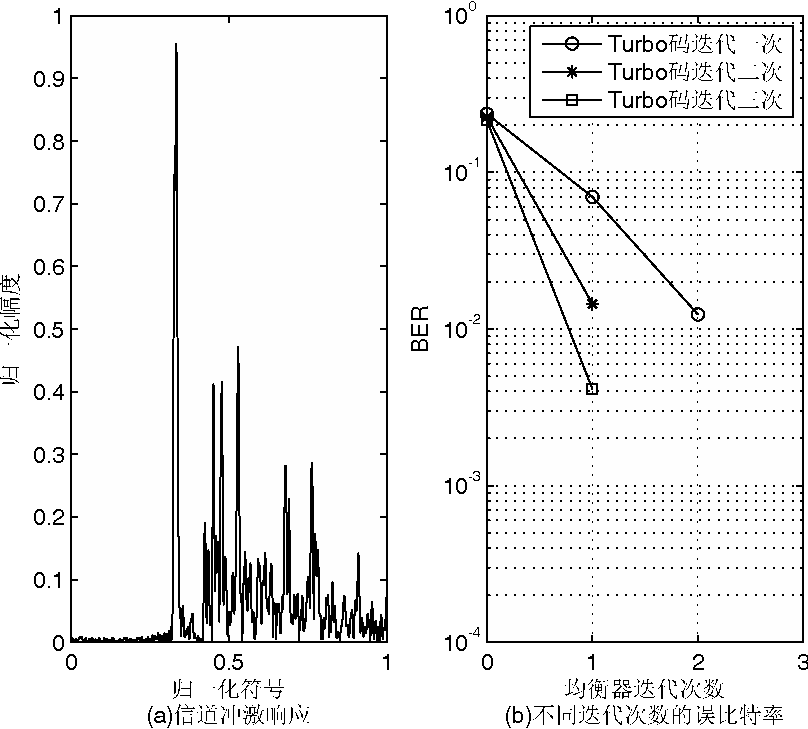
\includegraphics[width=0.9\textwidth]{images/result_1_2.pdf}
  \end{center}
  \caption{1052米处第二组数据包第一帧数据处理结果}
  \label{fig:6.10}
\end{figure}

\textbf{\sihao 2012年12月15日10:06:18数据 第一组} 

如图\ref{fig:6.11}为位置二(2617m)第一组第一帧数据的信道冲激响应和误码率曲线图,从图\ref{fig:6.11}(a)可以看出,此时的信道冲激响应的多径非常小,因此可以实现均衡器长度为2,相位估计器长度为2,且在均衡器迭代两次,而译码器迭代一次的情况下实现无差错译码。

联系位置一处两组数据的信道特征及误码率曲线图,可以知道,距离越远多径效应越小,从而需要的均衡器长度和信道估计器长度越小。

对图\ref{fig:6.11}(b)需要说明一下,Turbo码迭代三次的曲线在图中没有显示,是因为,均衡器迭代0次时,就可以实现无差错译码。

\begin{figure}[htb]
  \begin{center}
    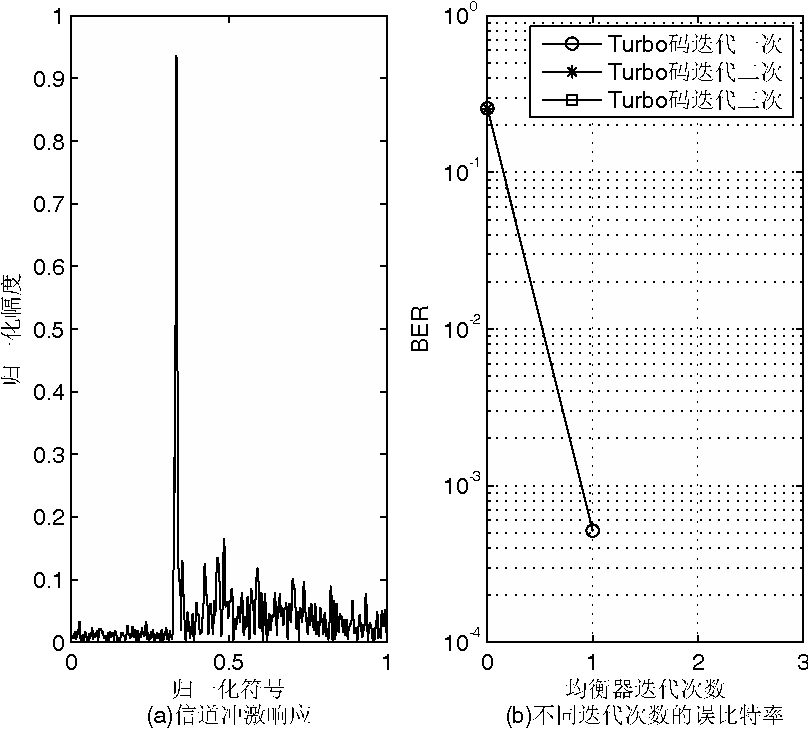
\includegraphics[width=0.9\textwidth]{images/result_2_1.pdf}
  \end{center}
  \caption{2617米处第一组数据包第一帧数据处理结果}
  \label{fig:6.11}
\end{figure}

\textbf{\sihao 2012年12月15日10:06:18数据 第二组} 

如图\ref{fig:6.12}为位置二(2617m)第二组第一帧数据的信道冲激响应和误码率曲线图,从图\ref{fig:6.11}(a)可以看出,此时的信道冲激响应的多径非常小,因此可以实现均衡器长度为2,相位估计器长度为2,且在均衡器迭代一次,而译码器迭代一次的情况下实现无差错译码。

相较于第一组数据中信道冲激响应,图\ref{fig:6.12}中的冲激响应多径的长度明显要小一些,但是多径的幅度要比第一组的大,从图\ref{fig:6.12}(b)的结果可以看出,多径的幅值并没有多均衡算法的性能产生影响,而多径的长度对性能的影响比较明显,这一结论与位置一处的两组数据所得出的结论一致。

此组数据的计算复杂度很低,可以实现无差错译码,一般深海信道多类似于图\ref{fig:6.11}(a)和\ref{fig:6.12}(a)中的信道冲激响应,有时比上述信道特性还要好,因此本文中的算法可以直接应用与深海通信中,但是浅海以及大部分湖试中,信道条件都比较差,信道的多径长度不可能很小,而时间反转技术的有点就是可以使信道聚焦,降低多径长度。

\begin{figure}[htb]
  \begin{center}
    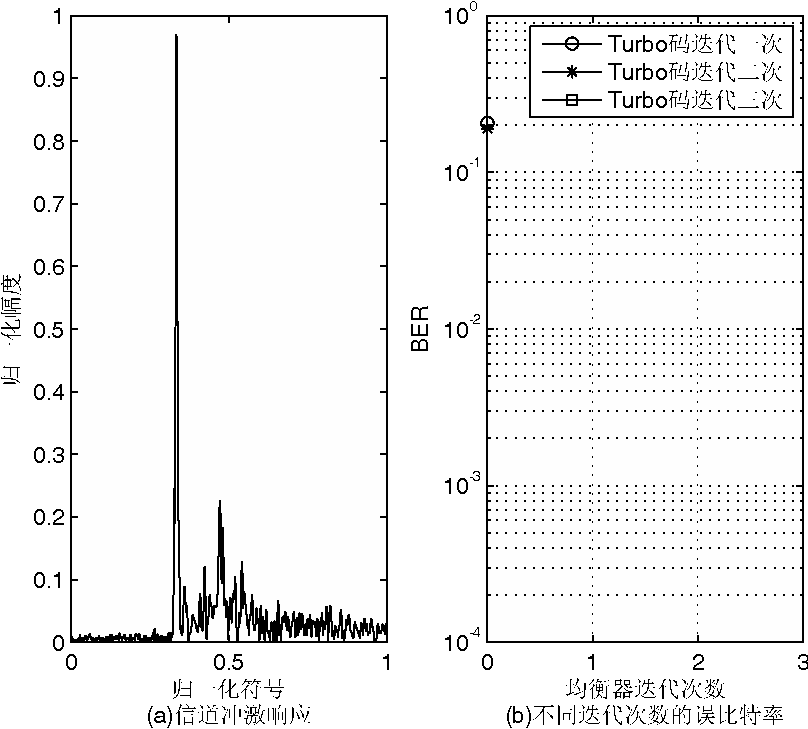
\includegraphics[width=0.9\textwidth]{images/result_2_2.pdf}
  \end{center}
  \caption{2617米处第二组数据包第一帧数据处理结果}
  \label{fig:6.12}
\end{figure}

\textbf{\sihao 2012年12月15日11:09:57数据 第一组} 

如图\ref{fig:6.13}为位置三(1763m)处第一组第一帧数据的信道冲激响应和误码率曲线图,图\ref{fig:6.13}(a)的信道冲激响应特性比位置一处要好,但是差于位置二处,因此,为了实现无差错译码,本组数据需要的均衡器长度为26,信道估计器长度为25,且需要均衡器迭代三次,译码器迭代一次。

\begin{figure}[htb]
  \begin{center}
    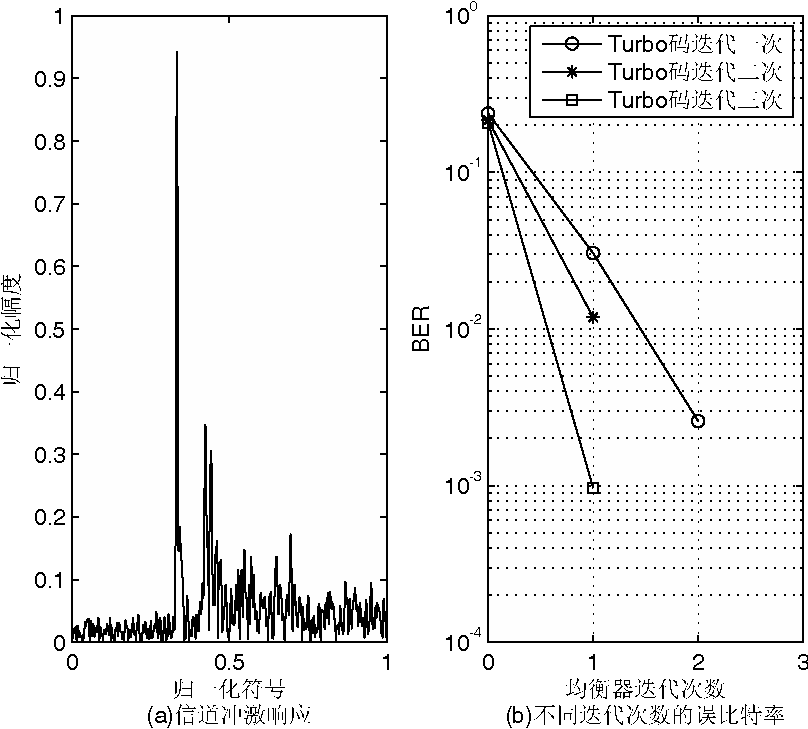
\includegraphics[width=0.9\textwidth]{images/result_3_1.pdf}
  \end{center}
  \caption{1736米处第一组数据包第一帧数据处理结果}
  \label{fig:6.13}
\end{figure}

\textbf{\sihao 2012年12月15日11:09:57数据 第二组} 

如图\ref{fig:6.14}为位置三(1763m)处第二组第一帧数据的信道冲激响应和误码率曲线图,图\ref{fig:6.14}(a)中的信道冲激响应的多径长度要大于图\ref{fig:6.13}(a),因此,为了为了实现无差错译码,本组数据需要的均衡器长度为35,信道估计器长度为32,且需要均衡器迭代三次,译码器迭代一次。这两组数据进一步验证位置一和位置二两组数据得出的结论,也即是:信道冲激响应的多径长度是影响均衡器性能的主要因素。

\begin{figure}[htb]
  \begin{center}
    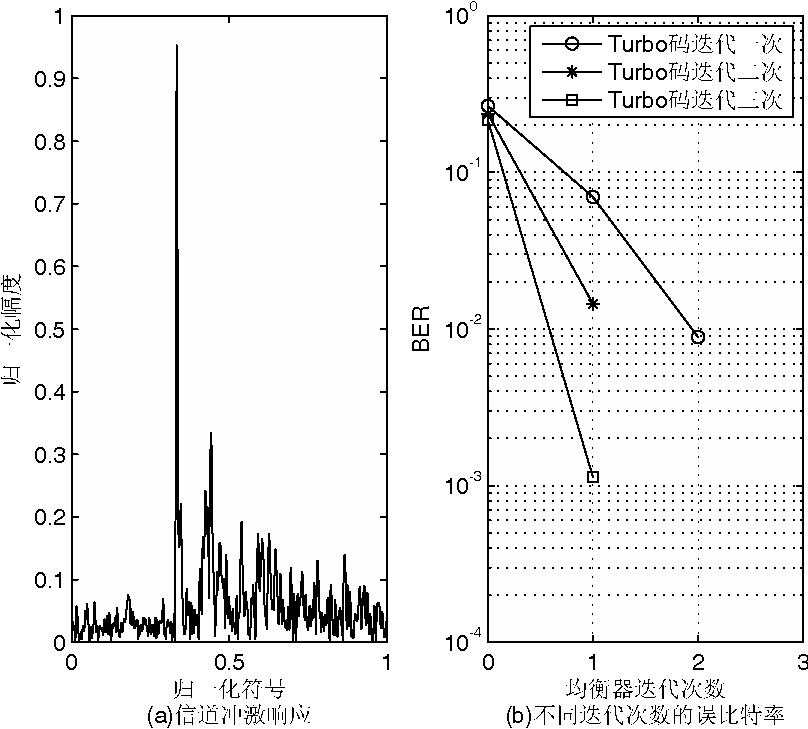
\includegraphics[width=0.9\textwidth]{images/result_3_2.pdf}
  \end{center}
  \caption{1736米处第二组数据包第一帧数据处理结果}
  \label{fig:6.14}
\end{figure}

\textbf{\sihao 2012年12月15日11:14:50数据 第一组} 

如图\ref{fig:6.15}为位置四(1645m)处第一组第一帧数据的信道冲激响应和误码率曲线图,图\ref{fig:6.15}(a)中的信道冲激响应比位置三处差,从各个位置处发送数据的环境分析,此时风浪较大,且船并没有抛锚固定而是随着风浪而运动,因此导致信道冲激响应较差。

此组数据为了实现无差错译码,需要的均衡器长度为45,信道估计器长度为44,且需要均衡器迭代三次,译码器迭代一次。

\begin{figure}[htb]
  \begin{center}
    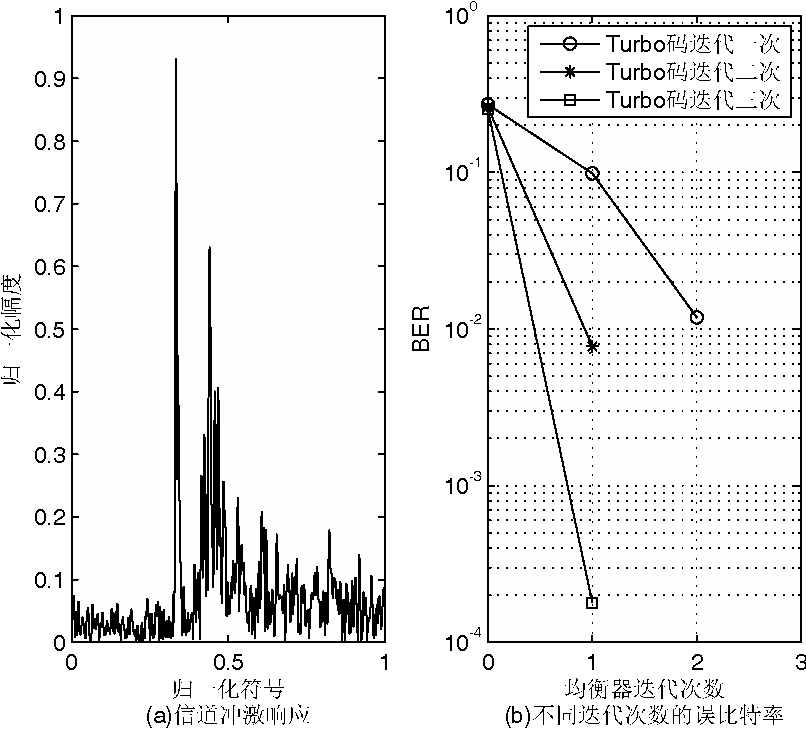
\includegraphics[width=0.9\textwidth]{images/result_4_1.pdf}
  \end{center}
  \caption{1645米处第一组数据包第一帧数据处理结果}
  \label{fig:6.15}
\end{figure}

\textbf{\sihao 2012年12月15日11:14:50数据 第二组} 

如图\ref{fig:6.16}为位置四(1645m)处第一组第一帧数据的信道冲激响应和误码率曲线图,比较图\ref{fig:6.13}(a)和\ref{fig:6.14}(a),可以发现,两者的信道多径长度基本一致,而图\ref{fig:6.14}(a)的多径幅值要比\ref{fig:6.13}(a)中的信道多径幅度大的多。比较\ref{fig:6.13}(b)和\ref{fig:6.14}(b),两者的误码率曲线基本一致。因此位置四处的两组数据进一步验证了多径长度是影响均衡器性能的主要因素这一结论。

\begin{figure}[htb]
  \begin{center}
    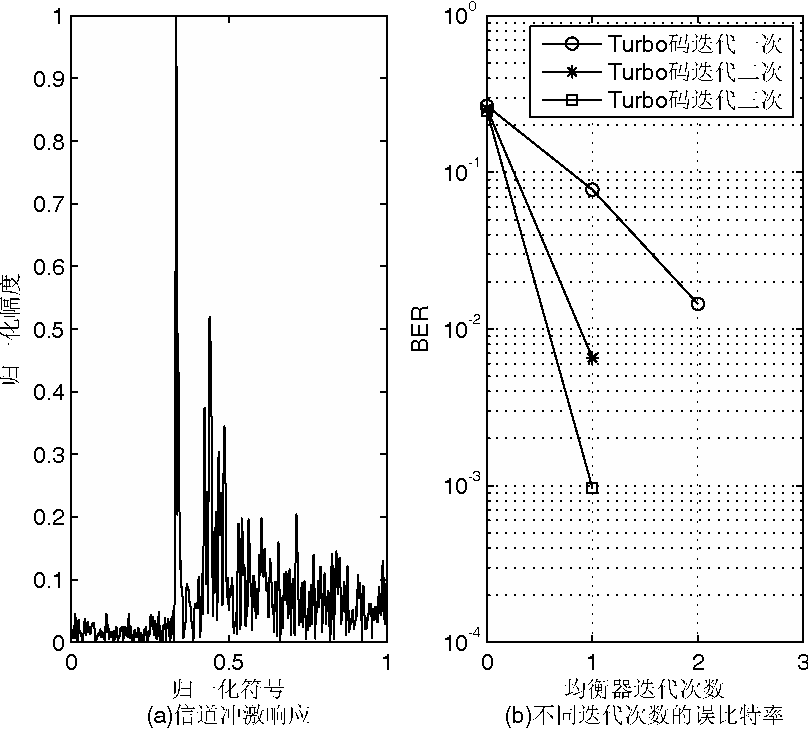
\includegraphics[width=0.9\textwidth]{images/result_4_2.pdf}
  \end{center}
  \caption{1645米处第二组数据包第一帧数据处理结果}
  \label{fig:6.16}
\end{figure}

虽然本文提出的基于先验信息MMSE准则的线性Turbo均衡算法能够无差错译码几乎所有位置所有组的所有帧数据,但是除了位置二处外,其他位置都要求均衡器和信道估计器的长度过长,从而引起运算复杂度过高,不能实现实时数据传输。
\section{本章小结}
本章首先介绍了湖试的试验环境及试验布置情况,而后对湖试地点的水声信道特性进行了分析,包括声速梯度和信道冲激响应。

在信道冲激响应分析的基础上,通过对湖试数据的Matlab处理,对算法性能作了进一步的分析、研究。数据处理针对水声相干通信系统的QPSK信号。湖试数据处理结果表明,本文研究的用于水声相干通信系统的软迭代信道估计算法及基于先验信息MMSE准则的线性Turbo均衡算法能够有效的处理多径信号并实现无差错传输。

通过湖试,我们验证了水声相干通信系统的原理和方案、信号处理系统的正确性、可行性以及系统硬件的可靠性,为下一步的海试和实际系统的交付使用做好了充分的准备。
%==========================================================================
%\end{document}
\clearpage{\pagestyle{empty}\cleardoublepage}
